\subsection{Main Window}
The main window is composed of several important views during any point in construction.  In the top left, we have the Material/Model Panel.  Using this panel, you can view the hierarchy of materials used to construct each assembly within the core.  Below that in the lower left is the Task Panel, which is different depending on what is selected in the Material/Model Panel. The 3D View is located on the right, which shows a 3-dimensional rendering of the selected component in the Material/Model Panel.  Refer to ~\ref{fig:mainwindow1} to see these labeled.

\begin{figure}[!htb]
\begin{center}
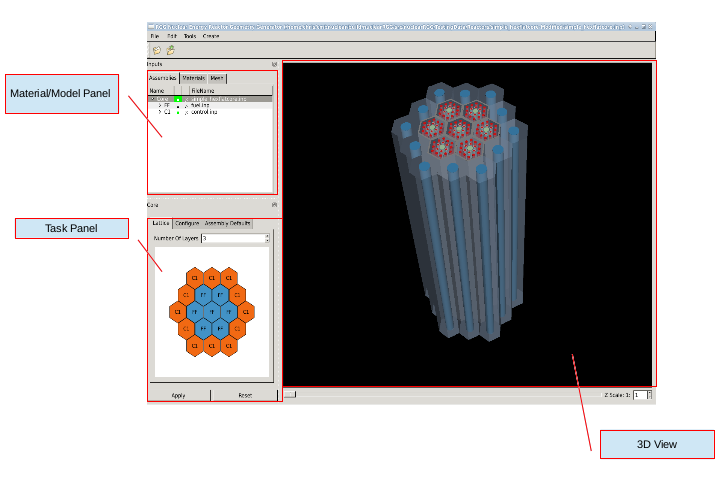
\includegraphics[width=0.6\linewidth]{Images/main-window-with-core-labeled-e1.png}
\caption{Three components are presented to the user upon loading an input (.inp) file or after building a core.}
\label{fig:mainwindow1}
\end{center}
\end{figure}


\subsection{Material/Model Panel}
The Material/Model Panel is a hierarchy of a reactor core, which is composed of assemblies, which are each composed of pins and ducts.  By clicking the drop-down arrow to the left of an object, you can see the parts which comprise the object.

The workflow of core generation can also be monitored through the Material/Model Panel.  Refer to ~\ref{fig:mmpanel1}.
\begin{figure}[!htb]
\begin{center}
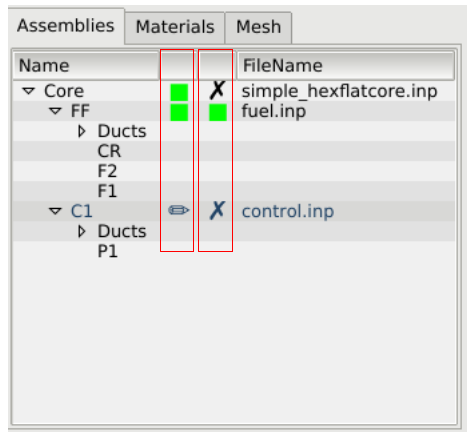
\includegraphics[width=0.6\linewidth]{Images/material-model-panel-labeled-e1.png}
\caption{Indicators in the Material/Model Panel are separated into two columns.}
\label{fig:mmpanel1}
\end{center}
\end{figure}


\subsubsection{Column 1 Indicators}
Column 1 indicates the state of the loaded assembly.  If the assembly has been saved, the indicator will be green.  If not, it will be marked with a pencil to indicate that it has been edited since the last save.

\subsubsection{Column 2 Indicators}
Column 2 indicates whether the current view of the assembly has been processed into a cubit (.cub) file.  If the .cub is newer than the .inp you loaded, this column will be green.  If not, there will be an ``x'' symbol there, indicating that this component has not yet been meshed.

\subsection{Task Panel}
\subsubsection{The Lattice Tab}
The Task Panel allows you to create a core out of the assemblies you have loaded or constructed.  Specify the number of layers (in a hexagonal core) or the dimensions (in a rectilinear core), and then right-click on each component to select an assembly.

\subsubsection{The Configure Tab}
This tab allows you to customize other parameters from the meshkit files which are not currently provided an interface in the GUI.  When building a hexagonal core, you should include a rotation of $$30^o$$ in each assembly, to prevent them from overlapping eachother.

\subsubsection{The Assembly Defaults Tab}
Here you can set whether the mesh you want to generate will be tetrahedral or hexagonal, and also change the default dimensions of the ducts comprising your core.  Changing these values will propagate all the way down to every component, so you can change it all in one place instead of adjusting the height of every duct in every assembly.

\subsection{Reactor Core View}
This is equivalent to the Task Panel view when a core is selected.  In addition to this, the entire core should be visible in the 3D view on the right, as in ~\ref{fig:mainwindow1}.

\subsection{Assembly View}
The Assembly View is visible when an assembly is selected in the Material/Model view.  An assembly is constructed from ducts and pins.  In the task panel, you can construct the assembly out of ducts and pins in the same way a core is constructed out of assemblies.  The dimensions of the assembly refer to how many ducts will be placed side-by-side.

\subsection{Duct View}
The Duct View is visible when a duct is selected in the Material/Model view.  In this mode, the 3D View shows the entire assembly.  The ``Position'' parameters can be used to edit the position of the duct in the render view, and also the thickness in the z direction.  The ``Thickness'' parameters can be used to edit the thickness in the x and y directions respectively. See Figure ~\ref{fig:ductedit1}.

\begin{figure}
\begin{center}
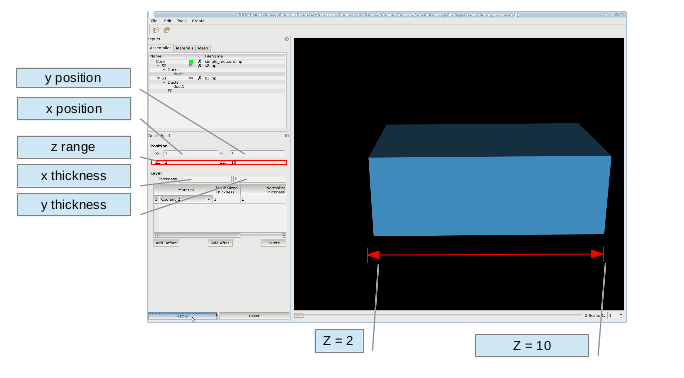
\includegraphics[width=0.6\linewidth]{Images/duct-editing-labeled.png}
\caption{The thickness and position of a duct can be edited from the Task Panel.}
\label{fig:ductedit1}
\end{center}
\end{figure}

\subsection{Pin Editing}
Edit a pin by selecting it in the Material/Model View.  It is useful to first change the key color and name, so that later it will be easily recognized while constructing your assembly.  See ~\ref{fig:pinedit1} for an example of the Task Panel when a pin is selected.

\begin{figure}
\begin{center}
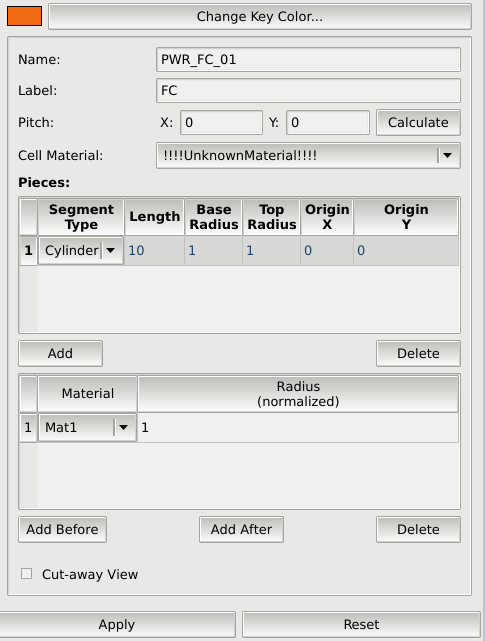
\includegraphics[width=0.6\linewidth]{Images/pin-editing.png}
\caption{A pin can be edited by selecting it in the Material/Model View.}
\label{fig:pinedit1}
\end{center}
\end{figure}


At this time there is only support for one piece to each pin.  This piece can be either a cylinder, when the top and bottom radii are identical, or a frustum, where they are different.

Once this is chosen, the material may be set.  A pin can be made out of more than one material, using the Material editor under the Pieces editor.  This enables you to set different layers of material with different radii.  See Figure ~\ref{fig:Rect6} for an example of this within the Rectangular Core tutorial.